\begin{figure*}[!htb]
	\centering
	%\hline
	\begin{subfigure}[t]{0.4\textwidth}
		\centering
		\caption{}
		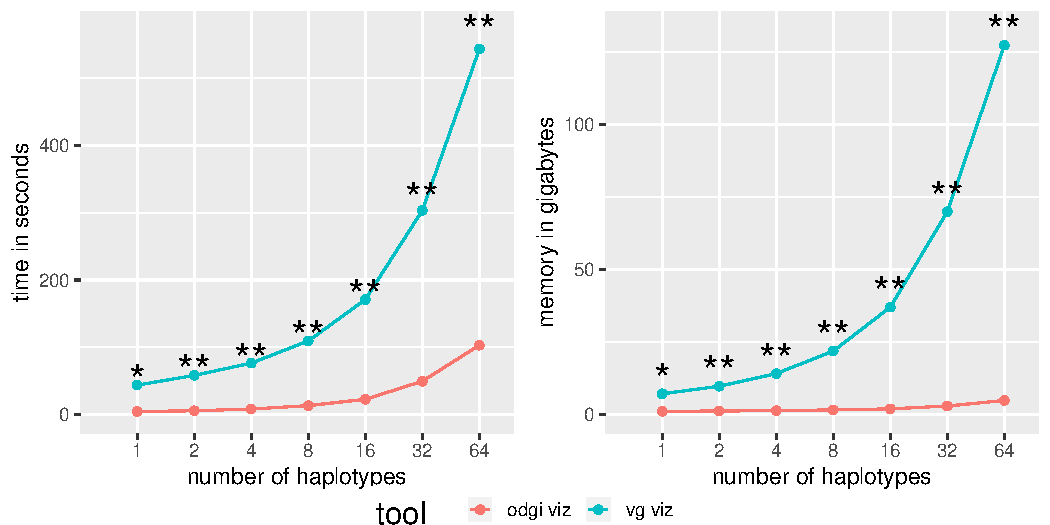
\includegraphics[width=\linewidth]{fig/performance/TODO_by_haps_eval_time_ram.pdf}
		\label{fig:haps_time_ram}
	\end{subfigure}
	\begin{subfigure}[t]{0.4\textwidth}
		\centering
		\caption{}
		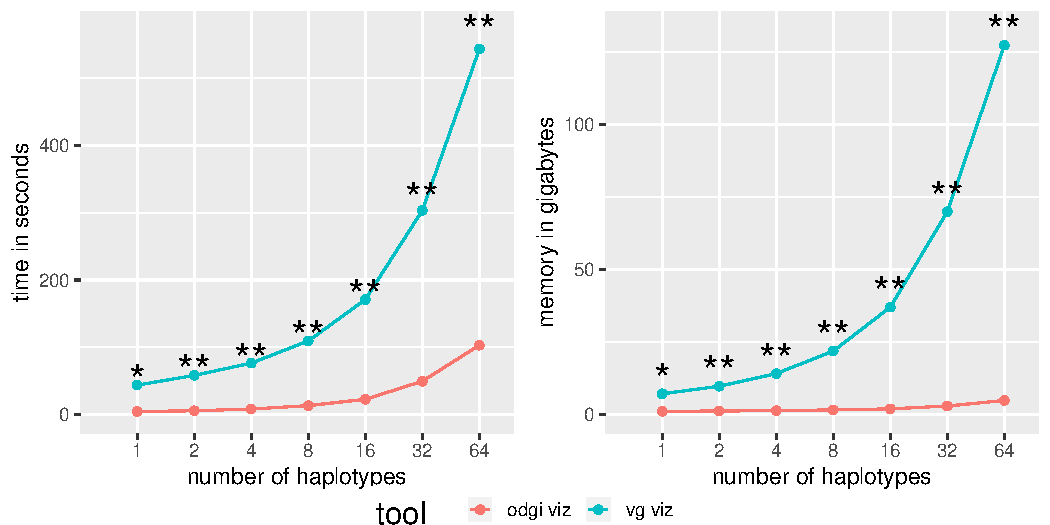
\includegraphics[width=\linewidth]{fig/performance/TODO_by_threads_eval_time_ram.pdf}
		\label{fig:threads_time_ram}
	\end{subfigure}
	%\smallskip
	\begin{subfigure}[t]{0.4\textwidth}
		\centering
		\caption{}
		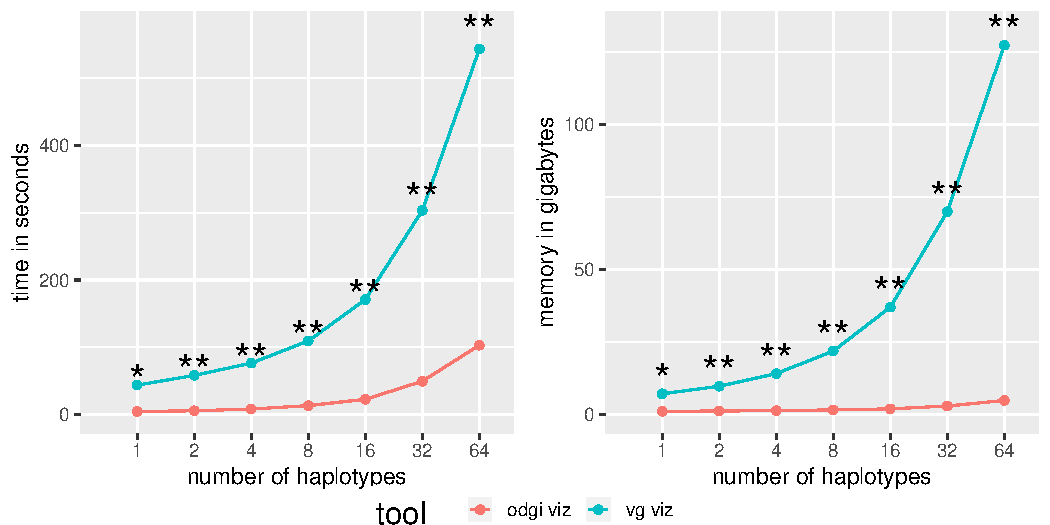
\includegraphics[width=\linewidth]{fig/performance/TODO_1d_alibi_time_ram.pdf}
		\label{fig:alibi}
	\end{subfigure}
	\begin{subfigure}[t]{0.4\textwidth}
		\centering
		\caption{}
		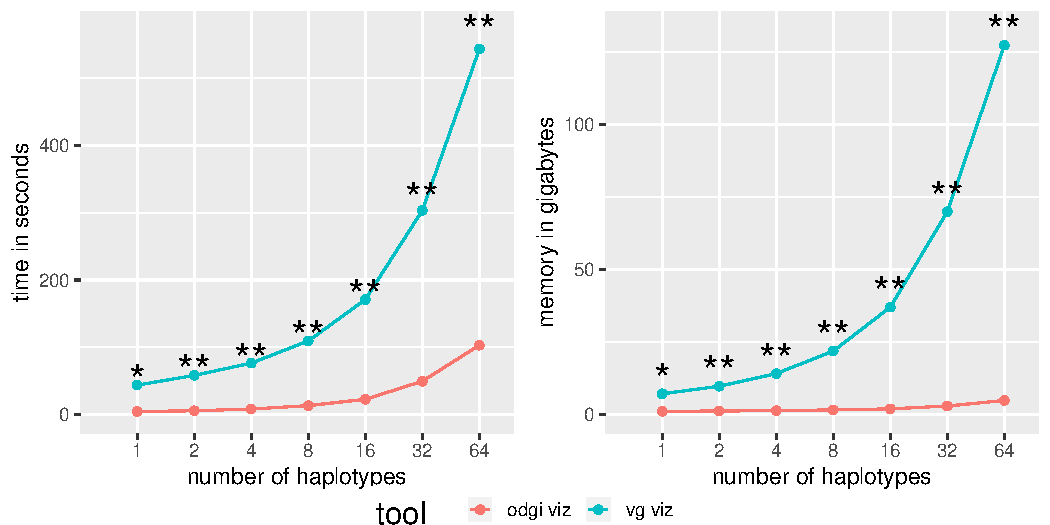
\includegraphics[width=\linewidth]{fig/performance/TODO_by_2d_draw_bandage_time_ram.pdf}
		\label{fig:bandage}
	\end{subfigure}
	\caption{
		Performance evaluations.
		\textbf{(a)} PG-SGD 1D and 2D by haplotypes. \textbf{(b)} PG-SGD 1D and 2D by threads. \textbf{(c)} PG-SGD vs. ALIBI. \textbf{(d)} PG-SGD + draw vs. BANDAGE.
	}
	\label{fig:performance}
\end{figure*}